\subsection{Dataset}
\label{dataset} In order to demonstrate the validity of the model
proposed in the previous sections, we compare its performance over a
data set against alternative strategies described in
Section~\ref{altstrats}. The data set consists of daily holdings of
five futures contracts denominated in non-USD currencies from
November 2003 to December 2012, for a total of 2115 observations.
Figure~\ref{prices} exhibits the future contracts prices and the
number of each contract held at any moment. These holdings are
exogeneous to our control; our aim is to find the optimal cash
margins given certain holdings of contracts denominated in foreign
currencies.
\begin{figure}[htbp]
    \centerline{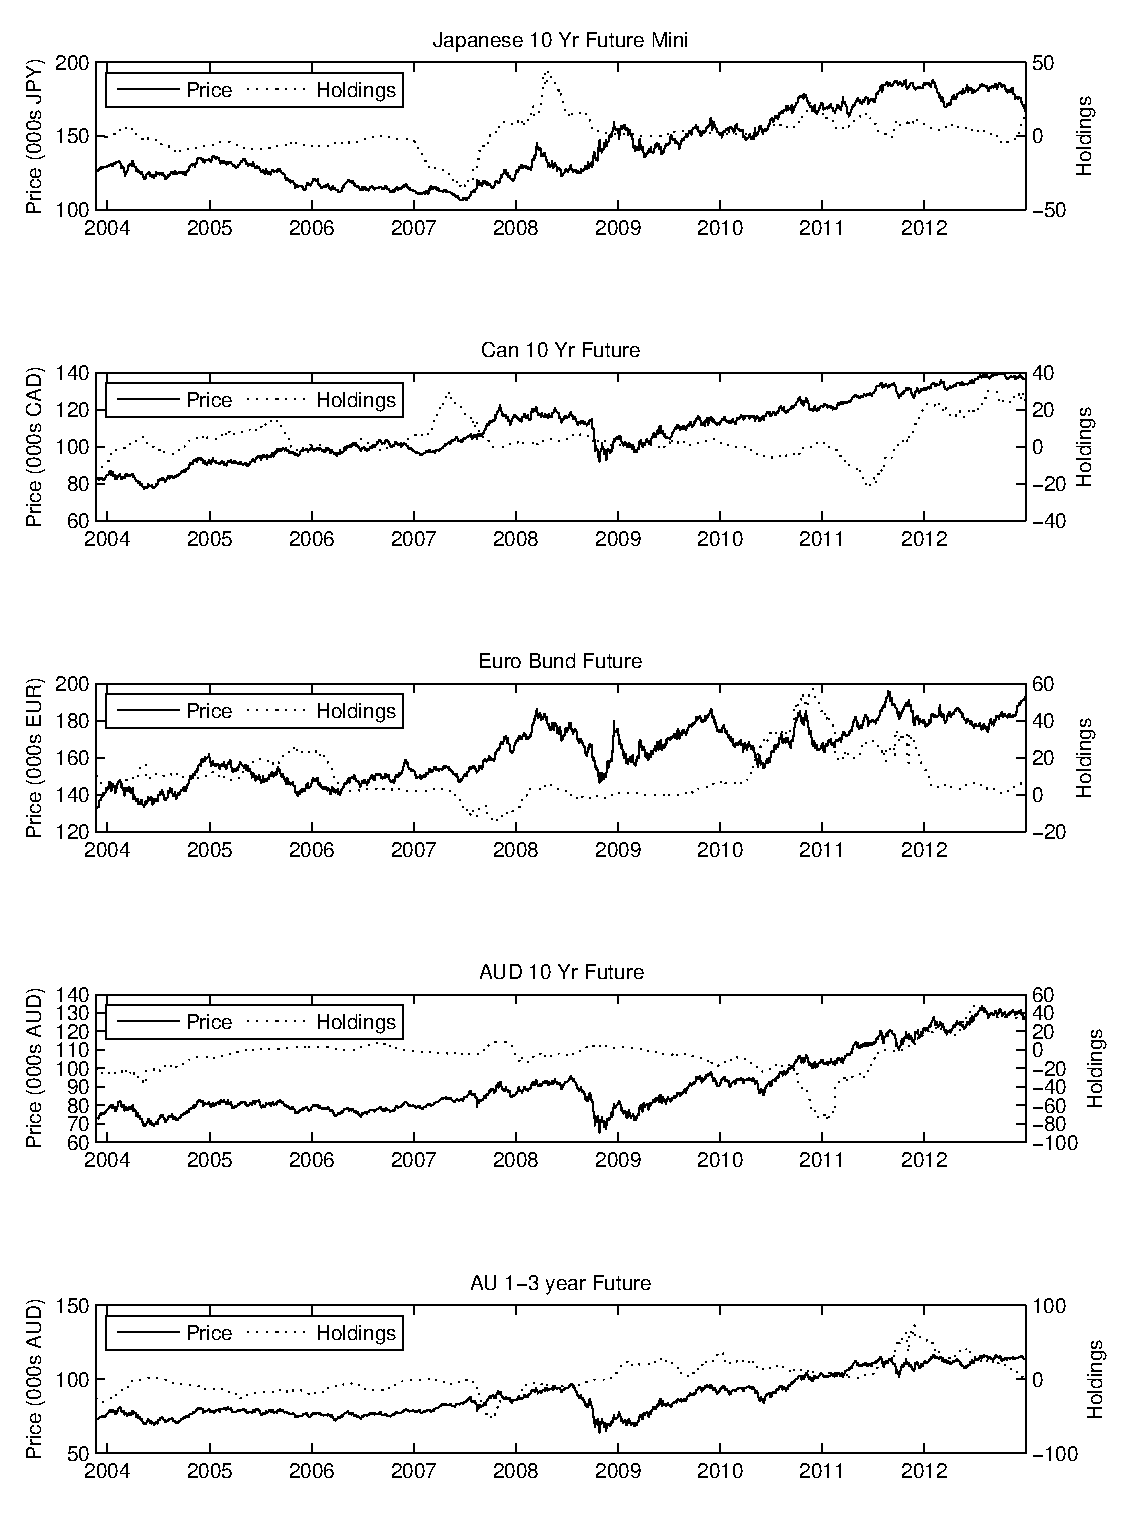
\includegraphics[scale=0.8]{contractsprices.eps}}
    \caption{Futures contracts prices and holdings}
\label{prices}
\end{figure}

A graphical test proposed by \cite{Gnanadesikan77} to test joint normality
was run on the data. If $\mathbf{X}=X_1, \ \ldots \ ,X_d$ is from a multivariate
Gaussian distribution, then
\begin{displaymath}
(\mathbf{X}_i-\bar{\mathbf{X}})' \ \Sigma \ (\mathbf{X}_i-\bar{\mathbf{X}}), \ i=1, \ \ldots \ ,N
\end{displaymath}
where $\Sigma$ is the covariance matrix of $\mathbf{X}$ have a $\chi^2_d$-distribution.
A QQ plot can then be used as a quick, ``litmus'' test of joint normality, as seen in
Figure~(\ref{mvQQplot}). Evidently joint normality has to be rejected.
\begin{figure}[htbp]
  \centerline{\includegraphics[scale=1]{mvQQplot.eps}}
   \caption{Graphical test of joint normality - QQ plot}
   \label{mvQQplot}
\end{figure}

